% Created by tikzDevice version 0.12.3.1 on 2021-12-14 20:20:29
% !TEX encoding = UTF-8 Unicode
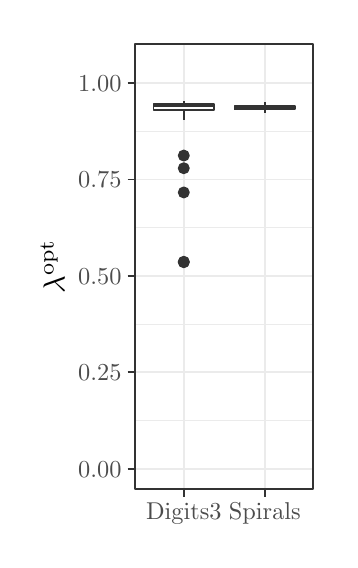
\begin{tikzpicture}[x=1pt,y=1pt]
\definecolor{fillColor}{RGB}{255,255,255}
\begin{scope}
\definecolor{drawColor}{RGB}{255,255,255}
\definecolor{fillColor}{RGB}{255,255,255}

\path[draw=drawColor,line width= 0.6pt,line join=round,line cap=round,fill=fillColor] ( -0.00, 16.11) rectangle (108.41,200.70);
\end{scope}
\begin{scope}
\definecolor{fillColor}{RGB}{255,255,255}

\path[fill=fillColor] ( 38.56, 34.33) rectangle (102.91,195.20);
\definecolor{drawColor}{gray}{0.92}

\path[draw=drawColor,line width= 0.3pt,line join=round] ( 38.56, 59.05) --
	(102.91, 59.05);

\path[draw=drawColor,line width= 0.3pt,line join=round] ( 38.56, 93.87) --
	(102.91, 93.87);

\path[draw=drawColor,line width= 0.3pt,line join=round] ( 38.56,128.69) --
	(102.91,128.69);

\path[draw=drawColor,line width= 0.3pt,line join=round] ( 38.56,163.52) --
	(102.91,163.52);

\path[draw=drawColor,line width= 0.6pt,line join=round] ( 38.56, 41.64) --
	(102.91, 41.64);

\path[draw=drawColor,line width= 0.6pt,line join=round] ( 38.56, 76.46) --
	(102.91, 76.46);

\path[draw=drawColor,line width= 0.6pt,line join=round] ( 38.56,111.28) --
	(102.91,111.28);

\path[draw=drawColor,line width= 0.6pt,line join=round] ( 38.56,146.11) --
	(102.91,146.11);

\path[draw=drawColor,line width= 0.6pt,line join=round] ( 38.56,180.93) --
	(102.91,180.93);

\path[draw=drawColor,line width= 0.6pt,line join=round] ( 56.11, 34.33) --
	( 56.11,195.20);

\path[draw=drawColor,line width= 0.6pt,line join=round] ( 85.36, 34.33) --
	( 85.36,195.20);
\definecolor{drawColor}{gray}{0.20}
\definecolor{fillColor}{gray}{0.20}

\path[draw=drawColor,line width= 0.4pt,line join=round,line cap=round,fill=fillColor] ( 56.11,116.24) circle (  1.96);

\path[draw=drawColor,line width= 0.4pt,line join=round,line cap=round,fill=fillColor] ( 56.11,150.21) circle (  1.96);

\path[draw=drawColor,line width= 0.4pt,line join=round,line cap=round,fill=fillColor] ( 56.11,154.79) circle (  1.96);

\path[draw=drawColor,line width= 0.4pt,line join=round,line cap=round,fill=fillColor] ( 56.11,141.46) circle (  1.96);

\path[draw=drawColor,line width= 0.4pt,line join=round,line cap=round,fill=fillColor] ( 56.11,116.41) circle (  1.96);

\path[draw=drawColor,line width= 0.6pt,line join=round] ( 56.11,173.47) -- ( 56.11,174.64);

\path[draw=drawColor,line width= 0.6pt,line join=round] ( 56.11,171.15) -- ( 56.11,167.81);
\definecolor{fillColor}{RGB}{255,255,255}

\path[draw=drawColor,line width= 0.6pt,line join=round,line cap=round,fill=fillColor] ( 45.14,173.47) --
	( 45.14,171.15) --
	( 67.07,171.15) --
	( 67.07,173.47) --
	( 45.14,173.47) --
	cycle;

\path[draw=drawColor,line width= 1.1pt,line join=round] ( 45.14,172.72) -- ( 67.07,172.72);

\path[draw=drawColor,line width= 0.6pt,line join=round] ( 85.36,172.79) -- ( 85.36,174.32);

\path[draw=drawColor,line width= 0.6pt,line join=round] ( 85.36,171.58) -- ( 85.36,169.99);

\path[draw=drawColor,line width= 0.6pt,line join=round,line cap=round,fill=fillColor] ( 74.39,172.79) --
	( 74.39,171.58) --
	( 96.32,171.58) --
	( 96.32,172.79) --
	( 74.39,172.79) --
	cycle;

\path[draw=drawColor,line width= 1.1pt,line join=round] ( 74.39,171.90) -- ( 96.32,171.90);

\path[draw=drawColor,line width= 0.6pt,line join=round,line cap=round] ( 38.56, 34.33) rectangle (102.91,195.20);
\end{scope}
\begin{scope}
\definecolor{drawColor}{gray}{0.30}

\node[text=drawColor,anchor=base east,inner sep=0pt, outer sep=0pt, scale=  0.88] at ( 33.61, 38.61) {0.00};

\node[text=drawColor,anchor=base east,inner sep=0pt, outer sep=0pt, scale=  0.88] at ( 33.61, 73.43) {0.25};

\node[text=drawColor,anchor=base east,inner sep=0pt, outer sep=0pt, scale=  0.88] at ( 33.61,108.25) {0.50};

\node[text=drawColor,anchor=base east,inner sep=0pt, outer sep=0pt, scale=  0.88] at ( 33.61,143.07) {0.75};

\node[text=drawColor,anchor=base east,inner sep=0pt, outer sep=0pt, scale=  0.88] at ( 33.61,177.90) {1.00};
\end{scope}
\begin{scope}
\definecolor{drawColor}{gray}{0.20}

\path[draw=drawColor,line width= 0.6pt,line join=round] ( 35.81, 41.64) --
	( 38.56, 41.64);

\path[draw=drawColor,line width= 0.6pt,line join=round] ( 35.81, 76.46) --
	( 38.56, 76.46);

\path[draw=drawColor,line width= 0.6pt,line join=round] ( 35.81,111.28) --
	( 38.56,111.28);

\path[draw=drawColor,line width= 0.6pt,line join=round] ( 35.81,146.11) --
	( 38.56,146.11);

\path[draw=drawColor,line width= 0.6pt,line join=round] ( 35.81,180.93) --
	( 38.56,180.93);
\end{scope}
\begin{scope}
\definecolor{drawColor}{gray}{0.20}

\path[draw=drawColor,line width= 0.6pt,line join=round] ( 56.11, 31.58) --
	( 56.11, 34.33);

\path[draw=drawColor,line width= 0.6pt,line join=round] ( 85.36, 31.58) --
	( 85.36, 34.33);
\end{scope}
\begin{scope}
\definecolor{drawColor}{gray}{0.30}

\node[text=drawColor,anchor=base,inner sep=0pt, outer sep=0pt, scale=  0.88] at ( 56.11, 23.32) {Digits3};

\node[text=drawColor,anchor=base,inner sep=0pt, outer sep=0pt, scale=  0.88] at ( 85.36, 23.32) {Spirals};
\end{scope}
\begin{scope}
\definecolor{drawColor}{RGB}{0,0,0}

\node[text=drawColor,rotate= 90.00,anchor=base,inner sep=0pt, outer sep=0pt, scale=  1.10] at ( 13.08,114.77) {$\lambda^\mathrm{opt}$};
\end{scope}
\end{tikzpicture}
